
%% Beispiel-Präsentation mit LaTeX Beamer im KIT-Design
%% entsprechend den Gestaltungsrichtlinien vom Februar 2025
%%
%% Siehe https://sdq.kastel.kit.edu/wiki/Dokumentvorlagen

%% Beispiel-Präsentation
\documentclass[]{sdqbeamer} 
 
%% Gruppenlogo, muss im Verezeichnis logos/ liegen
%% falls kein Gruppenlogo gewünscht, bitte \grouplogo{} aufrufen
\grouplogo{} 

%% Gruppenname und Breite (Standard: 89 mm)
\groupname{}
%\groupnamewidth{89mm}

% Beginn der Präsentation

%Information to be included in the title page:
\title{Combining Memory-Efficient Parallel SAT Solving and Distributed Clause Sharing}
\subtitle{Master Thesis}
\author{Ruben Götz}

\date[11.\,9.\,2025]{11. September 2025}

% Literatur 
 
\usepackage[citestyle=authoryear,bibstyle=numeric,hyperref,backend=biber]{biblatex}
%\addbibresource{slides.bib}
\bibhang1em

\usepackage{lipsum}
\usepackage{booktabs}
\usepackage{subcaption}
\usepackage{xcolor}
\usepackage{xurl}

% 20-25 Minuten ist die Norm für einen Mastervortrag. 
% Eine kurze Einleitung für Menschen, die SAT Solving 
% schonmal gehört haben, ganz kurz der relevante 
% Stand der Technik, deine Contributions als Hauptteil 
% und die wichtigsten Ergebnisse aus der Evaluation 
% (dem kannst du denke ich viel Gewicht geben, weil 
% das dann auch den Schwerpunkt deiner MA spiegelt). 


%\begin{minipage}{0.5\textwidth}
%...
%\end{minipage}%
%\begin{minipage}{0.5\textwidth}
%...
%\end{minipage}%

% 1: Anderes Titelbild vielleicht?
% x 2: exemplary
% x 3: Use Cases (+Bilder)
% x 4: Es ist mir in der SAT Community ein wichtiges Anliegen zu verbreiten, dass Solver à la MallobSat eben nicht "Portfolio mit ein bisschen Clause Sharing" sind sondern "Clause Sharing Solver with some added diversification over solver threads". Insbes. ist erwiesen, dass clause sharing nicht einfach Effizienz verbessert sondern das primäre Standbein für die Skalierbarkeit ist. Evtl kannst du diese Zwischentöne berücksichtigen
% x 5: 1st mention of Gimsatul: Zitat (Autoren, Jahr) dahinter. Generell auch Highlighting, z.B. fett, für wichtige Wörter?
% x 6: "[Schreiber&Sanders. 2023]" => "[Schreiber&Sanders 2024]". Ebenso kein Punkt bei Slide7
% 10: erklärst du internal vs. external hier?
% x 12: Details zum rechten Plot: Scale, Setup (Kissat / Gimsatul / ...)? Solche Dinge mach ich gerne in kleiner grauer Schrift unter den Plot, dann schnallt jeder dass es keine essentiellen Infos sind aber man kann sie tz. lesen
% x 13: "Benchmarks" Komisch formuliert. Die Benchmarks kommen von der International SAT Competition 2024. Bezogen hast du sie via GBD (aber das ist ein Detail).
% x 15: Speedup über welche Baseline?
% x 16: Gimsatul vs. Kissat deutlich machen
% x 17ff: Ich finde nicht, dass du unter den Plots so volle Captions brauchst, ich würde eher wie zu 12 angedeutet Basic Infos Schlagwort-artig in grau drunterschreiben (hier z.B. die Scale)
% x 18: Titel fehlt
% x 19 und vorherige: Titel der Folie evtl. pro Slide weiter konkretisieren?
% x 22: hier besonders, was ich zu 17 geschrieben hab

\begin{document}

%Titelseite
\begin{frame}[title white vertical, picture=images/palladio_bauplan]
	\titlepage
\end{frame}

%%%%%%%%%%%%%%%%%%%

\section{Introduction}
\begin{frame}{Introduction}
    \begin{block}{SAT Solving}
        Given a Boolean formula (usually in CNF):
        \begin{itemize}
            \item Decide whether Formula is SAT
            \item Give assignment if Formula is SAT
        \end{itemize}
    \end{block}

    \begin{exampleblock}{$F = (a \lor b) \land (\lnot a \lor c \lor d)$}
        Is SAT for exemplary assignment $a = false, b = true, c = false, d = false$
    \end{exampleblock}
\end{frame}

\urldef{\sudokuurl}\url{https://sudoku.com/}
\urldef{\cryptourl}\url{https://thebestvpn.com/cryptography/}
\urldef{\aiurl}\url{https://medium.com/}
\begin{frame}{Introduction}
    \begin{minipage}{.45\textwidth}
        \begin{block}{Usecases}
            \begin{itemize}
                \item Hardware and Software verification
                \item Automated Planning
                \item Scheduling
                \item Cryptoanalysis
                \item (explainable) AI
                \item Theorem Proving
                \item $\cdots$
            \end{itemize}
            \end{block}
    \end{minipage}
    \hfill
    \begin{minipage}{.45\textwidth}
        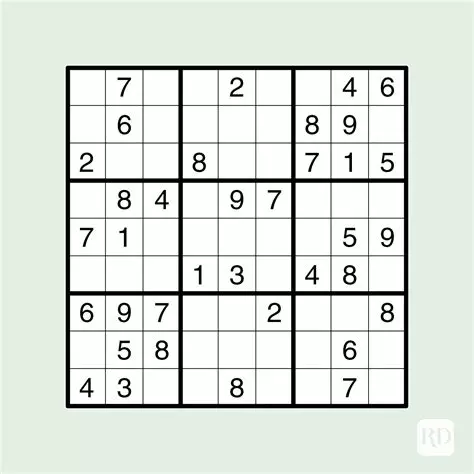
\includegraphics[scale=.075]{images/Sudoku.png}\footnote{\sudokuurl}
        
\includegraphics[scale=.35]{images/Cryptography.png}\footnote{\cryptourl}
        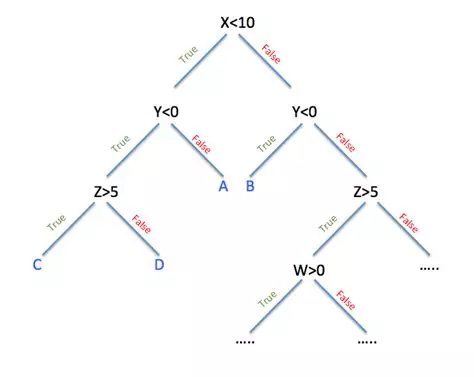
\includegraphics[scale=.35]{images/decition_tree.png}\footnote{\aiurl}
    \end{minipage}
\end{frame}

%%%%%%%%%%%%%%%%%%%%%%%%%%

\section{State of the Art}
\begin{frame}{State of the Art}
    \begin{block}{Serial SAT solvers}
        \begin{itemize}
            \item Mostly based on CDCL algorithm
            \item i.e. learns conflict clauses
        \end{itemize}
    \end{block}

    \begin{block}{Parallel SAT solvers}
        \begin{itemize}
            \item Search Space Partitioning: Divide problem into disjoint subspaces
            \item Portfolio Solvers: Run multiple diverse serial solvers in parallel
            \begin{itemize}
                \item Increase efficiency by sharing clauses
                \item Distributed SAT solving is on the rise
                \item Annual SAT competition includes cloud track since 2020
                % \item MallobSat
            \end{itemize}
            \item[$\Rightarrow$] Clause Sharing Solver
        \end{itemize}
    \end{block}
\end{frame}

\begin{frame}{State of the Art}
    \begin{block}{Memory-Efficient SAT solving}
        \begin{itemize}
            \item Most research focuses on runtime
            \item Running independent solver engines comes with inherent memory redundancy
            \item[$\Rightarrow$] Gimsatul utilizes shared clauses in Memory [\href{https://arxiv.org/pdf/2207.13577}{Fleury\&Biere~2022}]
        \end{itemize}
    \end{block}

    \begin{block}{Contributions}
        \begin{itemize}
            \item Integrate Gimsatul into MallobSat to combine memory efficiency with scalability
            \item Implement \textit{search only} approach [\href{https://satres.kikit.kit.edu/papers/2025-sat-streamlining-pre.pdf}{Schreiber et al.~2025}]
            \item Evaluate approach experimentally
        \end{itemize}
    \end{block}
\end{frame}

% Ich hab Mallob jetzt als 2023 anegeben, aber das Paper aus 2024 verlinkt
\begin{frame}{How MallobSat Works [\href{https://www.jair.org/index.php/jair/article/download/15827/27072}{Schreiber\&Sanders~2024}]}
    \center
    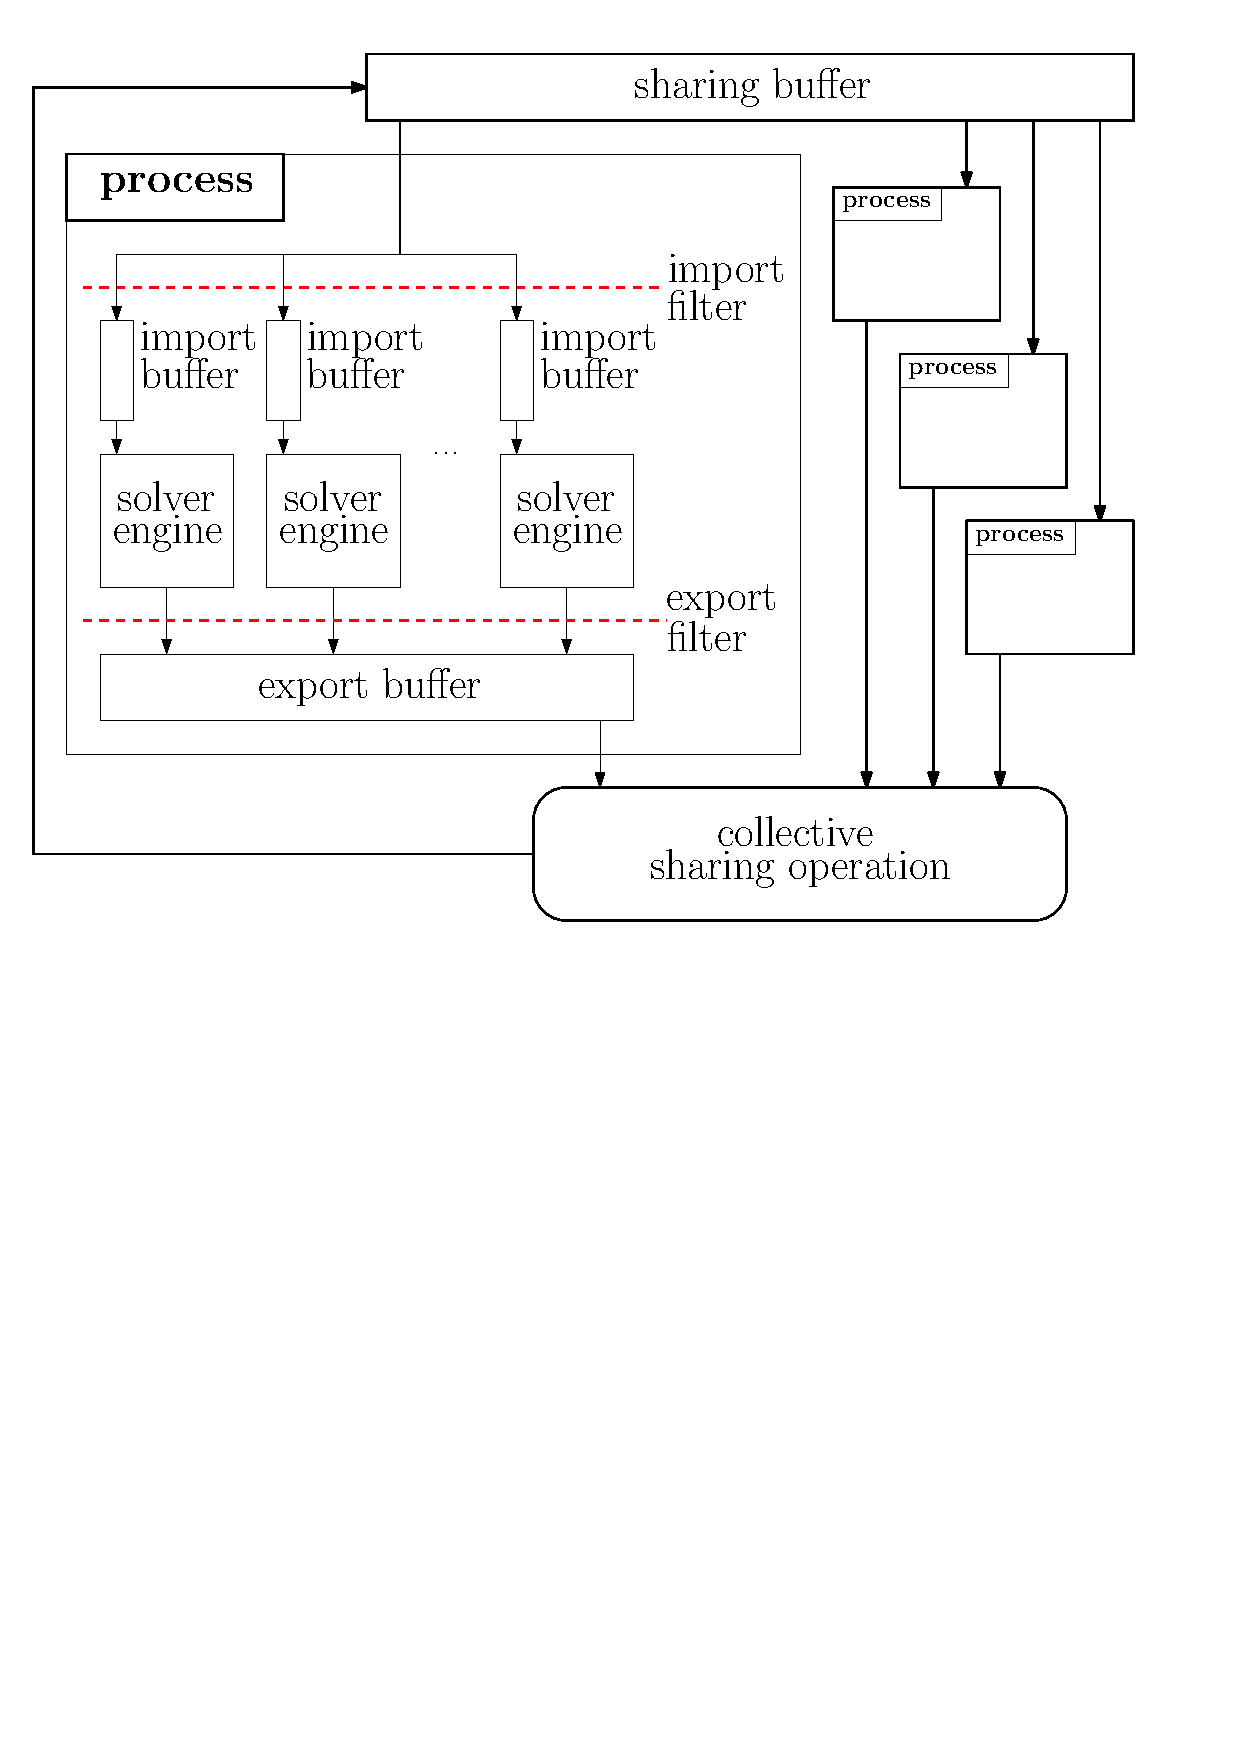
\includegraphics[scale=.8]{figures/mallob_architecture.pdf}
\end{frame}

\begin{frame}{How Gimsatul Works [\href{https://arxiv.org/pdf/2207.13577}{Fleury\&Biere~2022}]}
    \center
    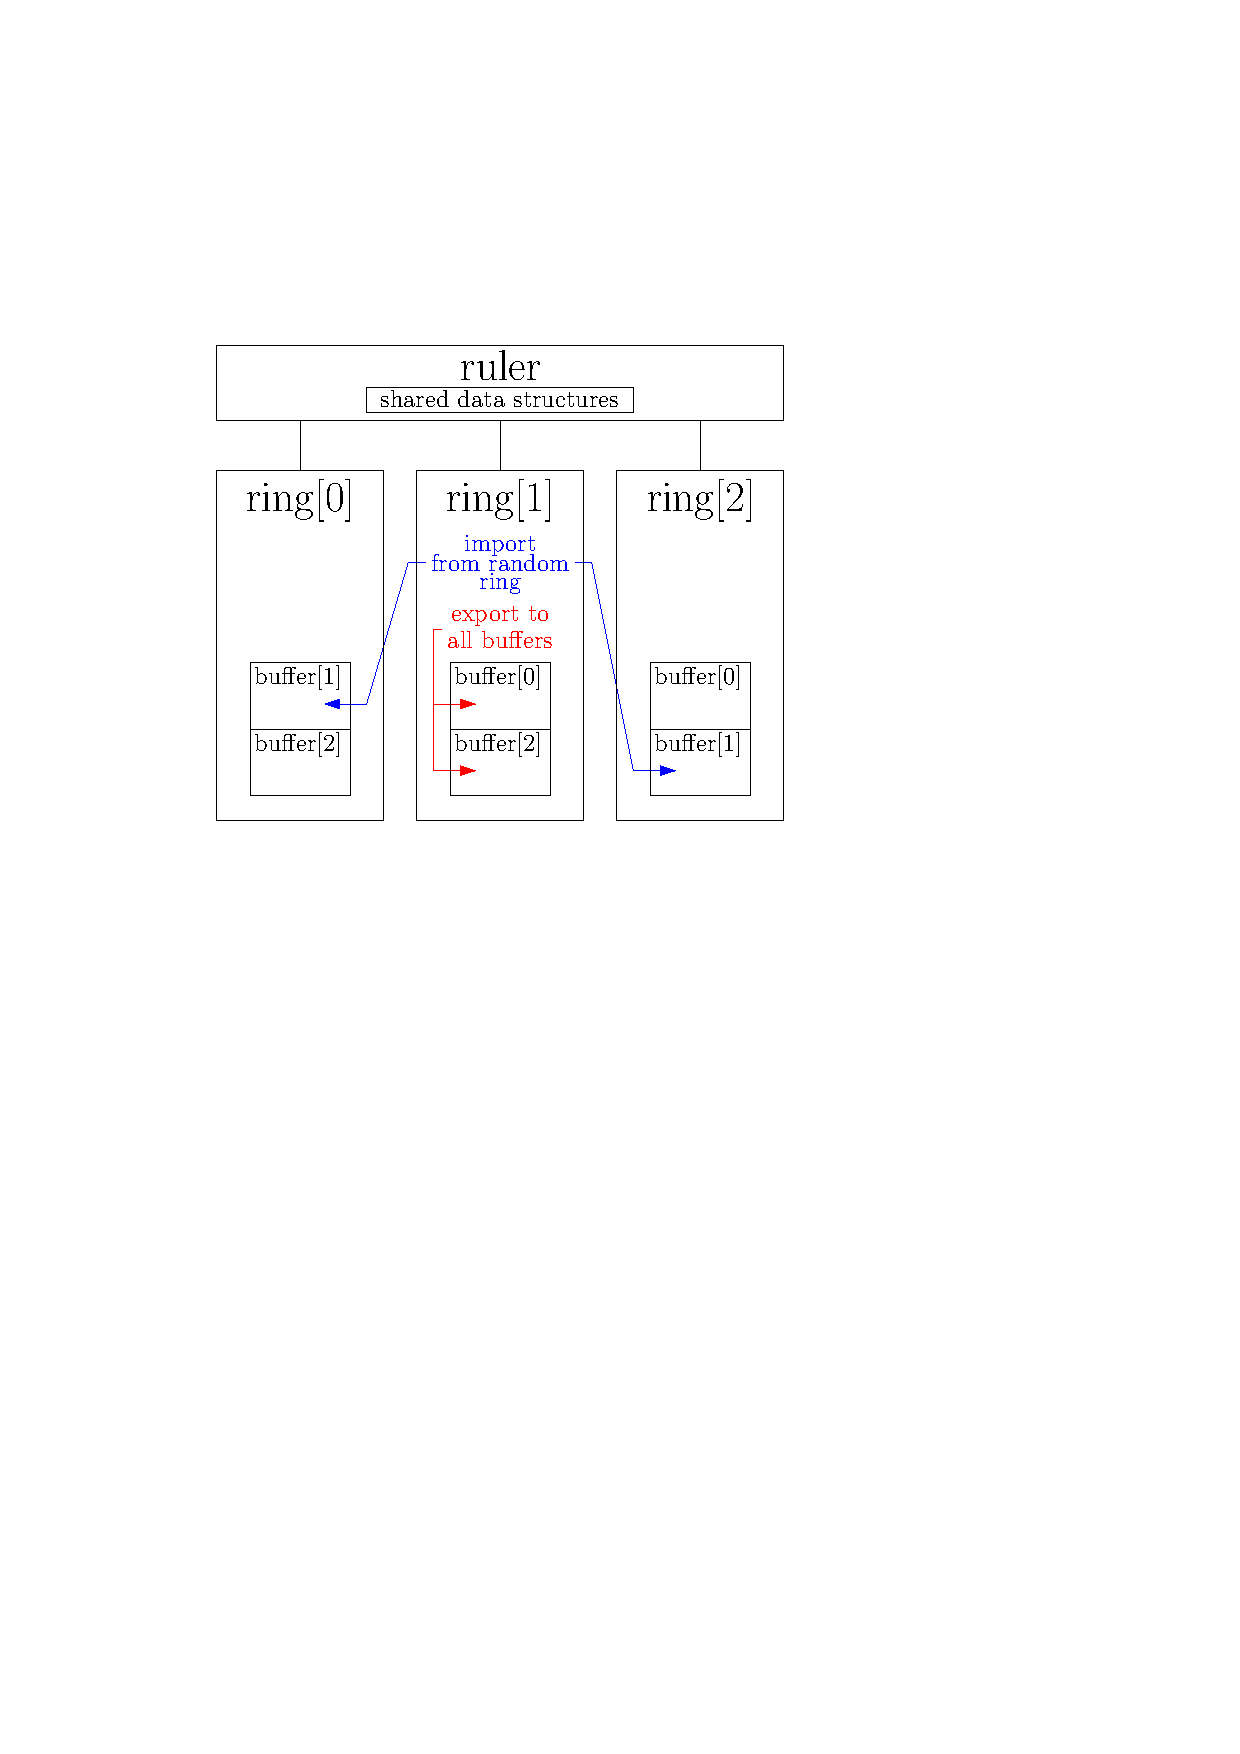
\includegraphics[scale=1.5]{figures/gimsatul_architecture.pdf}
\end{frame}

%%%%%%%%%%%%%%%%%%%%%%%%%%%%%%55

\section{Our Architecture}
\begin{frame}{Our Architecture}
    \center
    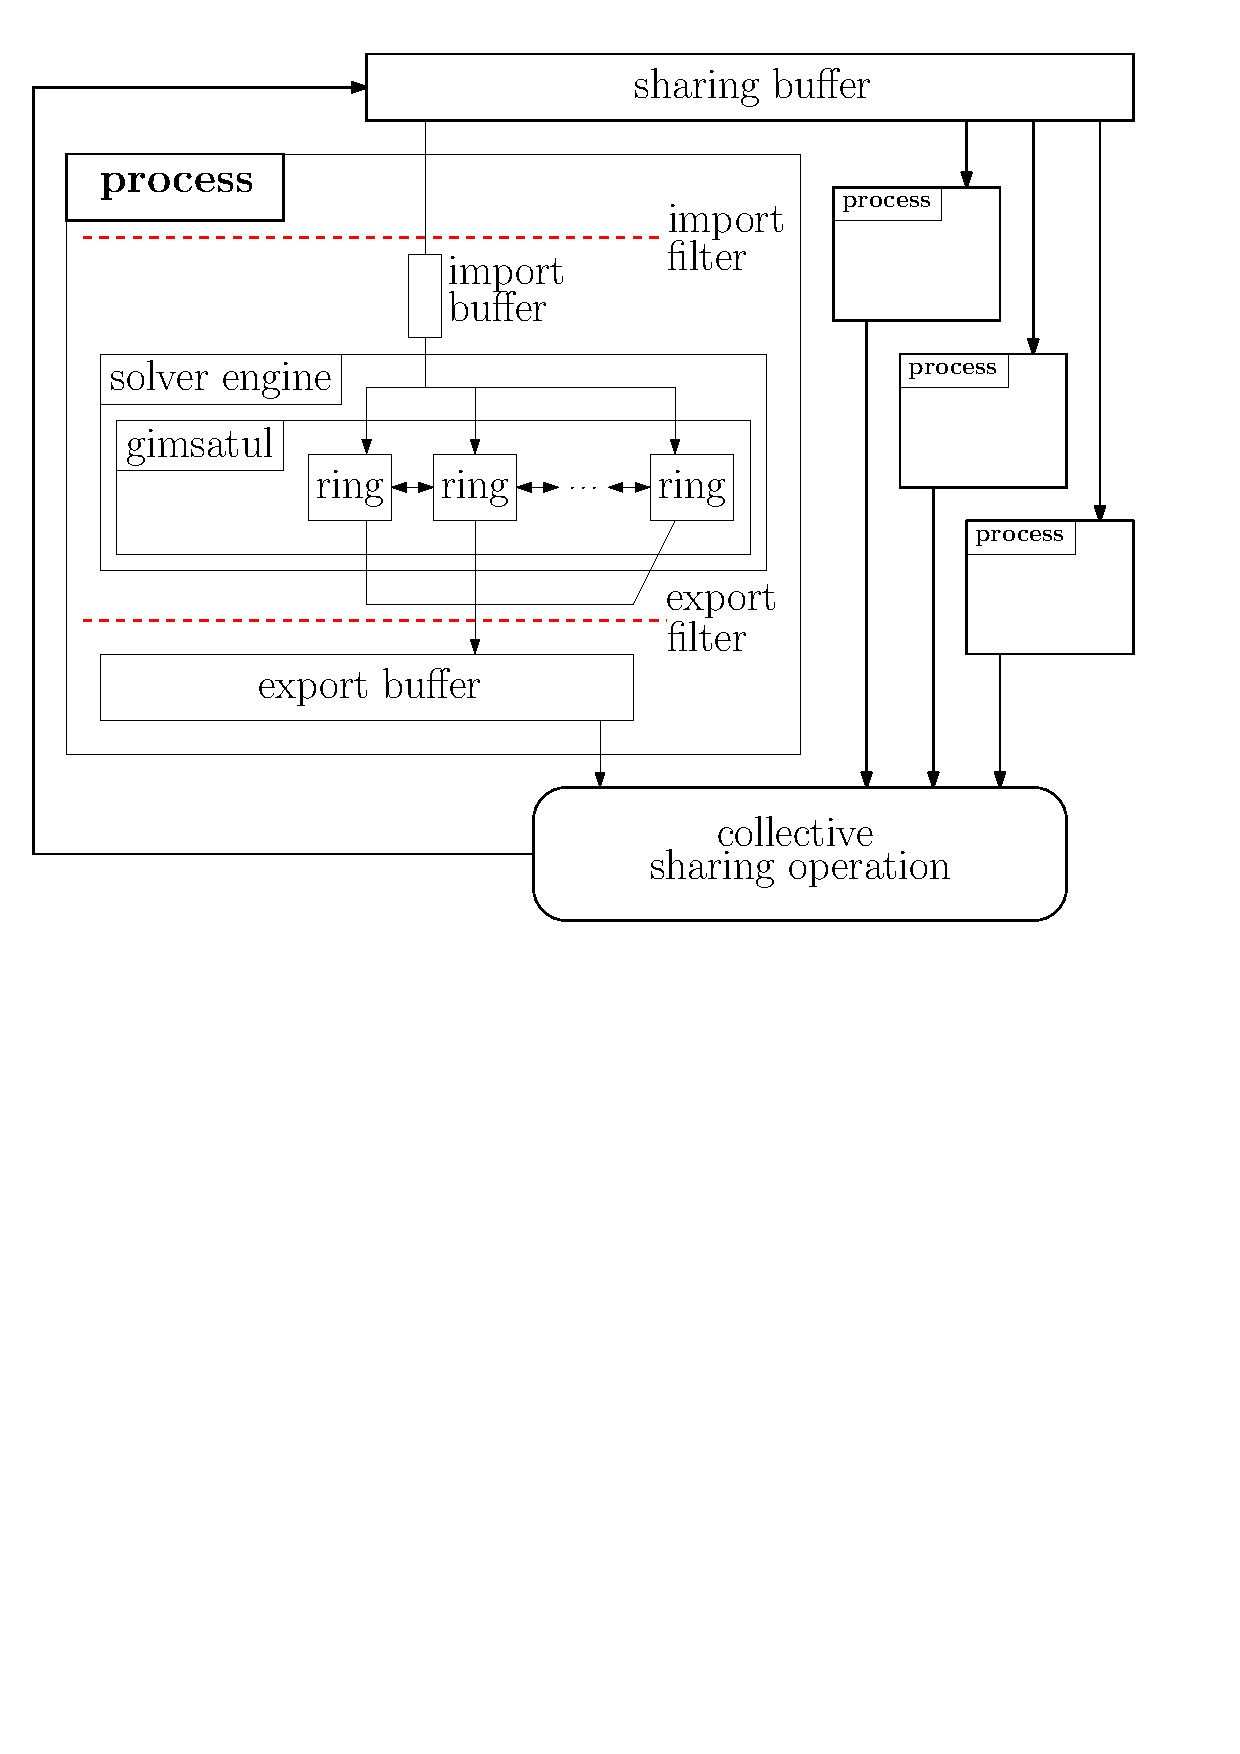
\includegraphics[scale=.8]{figures/architecture.pdf}
\end{frame}

\begin{frame}{Our Architecture}
    \begin{block}{Creating the Solver Engine}
        If Gimsatul is part of portfolio:
        \begin{itemize}
            \item Accumulate all $t'$ threads, that are defined to be Gimsatul
            \item Run Gimsatul with $t'$ threads
            \item MallobSat process runs with $t$ threads and $t - t' + 1$ solver engines
            \item extend Gimsatul's diversification
        \end{itemize}
    \end{block}
\end{frame}

\begin{frame}{Our Architecture}
    \begin{block}{Clause Export}
        \begin{itemize}
            \item All rings export externally if they export internally
            \item MallobSat's clause sharing mechanisms elegantly handles...
            \begin{itemize}
                \item[...] Clause filtering
                \item[...] Avoiding redundant clause sharing
            \end{itemize}
        \end{itemize}
    \end{block}

    \begin{block}{Clause Import}
        \begin{itemize}
            \item All rings import independently
            \item If there are conflicts, importing is skipped
            \item A ring imports at most as many clauses as there are rings in its Gimsatul instance
        \end{itemize}
    \end{block}
\end{frame}

\begin{frame}{Our Architecture}
    \begin{block}{Diversification}
        Added \textit{sparse random variable phases} on top of Gimsatuls native diversification:
        \begin{itemize}
            \item Flip phases of random variables
            \item $p = 1 / e$ for $e$ engines in total
            \item implemented as $p = 1 / (t' * p)$ for $t'$ rings and $p$ processes
        \end{itemize}
    \end{block}
\end{frame}

\begin{frame}{Our Architecture}
    \begin{minipage}{0.45\textwidth}
        \center
        \begin{block}{Search Only}
            \begin{itemize}
                \item Proposed by Schreiber, Rigi-Luperti \& Biere in 2025
                \item Deactivate pre- and inprocessing
                \item Run single dedicated preprocessing job in the beginning
                \item Replace jobs with preprocessed formula over time
            \end{itemize}
        \end{block}
    \end{minipage}%
    \hfill
    \begin{minipage}{0.45\textwidth}
        \center
        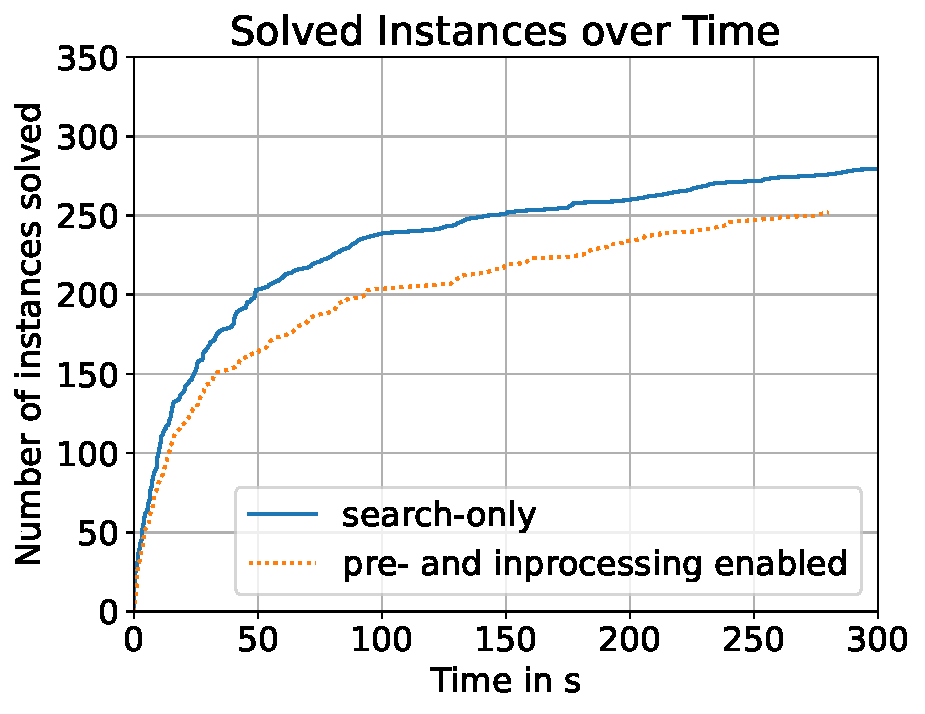
\includegraphics[scale=.8]{plots/config_compare/search_only_compare.pdf}\\
        \textcolor{gray}{Same configuration of one Gimsatul instace per node. Once with \textit{search only} and once with pre- and inprocessing}
    \end{minipage}%

\end{frame}

%%%%%%%%%%%%%%%%%%%%%%%%%%%%%%%%%%

\section{Experimental Evaluation}
\begin{frame}{Benchmarks \& Configuration}
    \begin{block}{Benchmarks}
        We used the benchmarks from the international SAT Competition 2024. Specifically, the track \textit{main\_2024}.
    \end{block}

    \begin{block}{Configuration}
        \begin{itemize}
            \item Experiments done on SuperMUC
            \begin{itemize}
                \item 1 node contains 48 cores (96 Hardware threads)
                \item used up to 16 nodes (768 cores)
            \end{itemize}
            \item 1 Gimsatul instance per node
            \item 48 threads per node
            \item Search Only approach
        \end{itemize}
    \end{block}
\end{frame}

\begin{frame}{Runtime}
    \center
    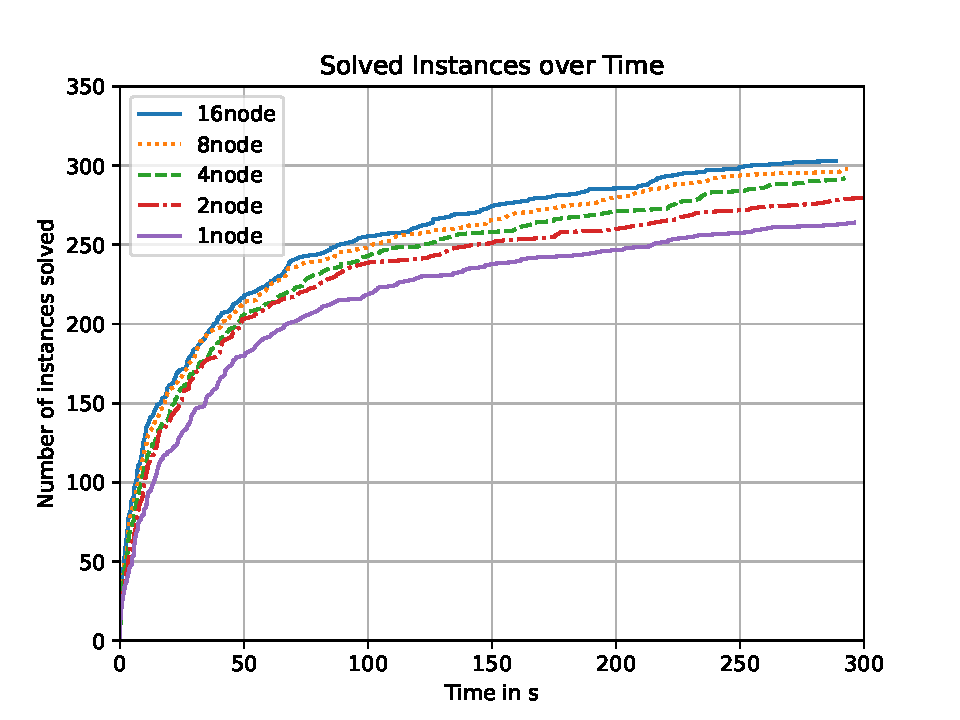
\includegraphics[scale=1]{plots/cumulative_runtime/scalability_gim.pdf}
\end{frame}

\begin{frame}{Speedups over Serial Kissat [\href{https://cca.informatik.uni-freiburg.de/papers/BiereFallerFazekasFleuryFroleyksPollitt-SAT-Competition-2024-solvers.pdf}{Biere et al.~2024}]}
    \begin{minipage}{.45\textwidth}
        \noindent
        \center
        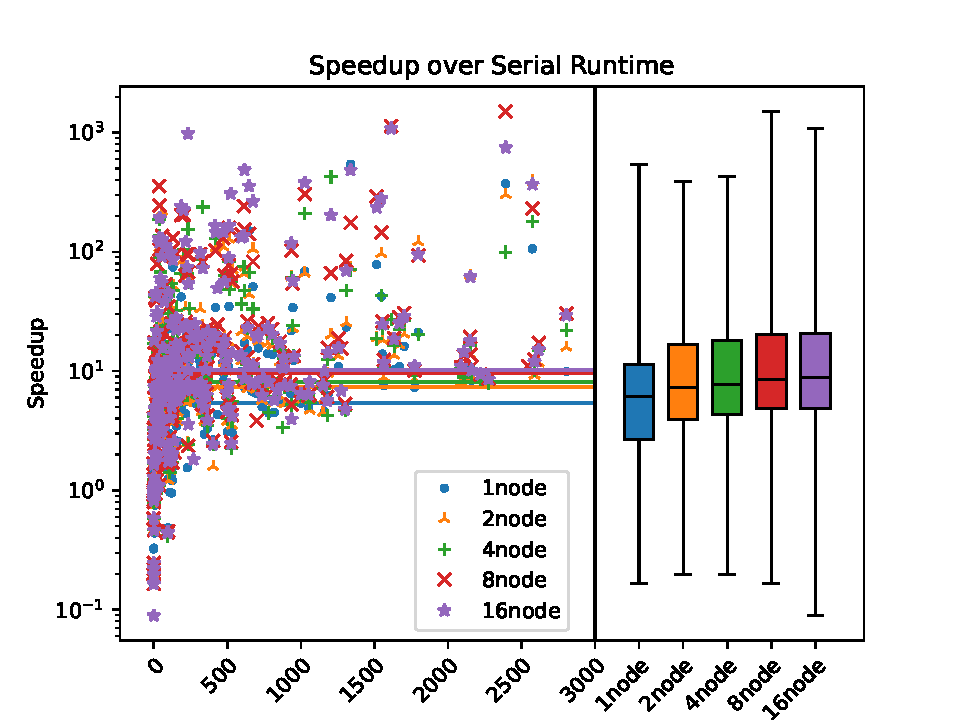
\includegraphics[scale=.6]{plots/speedups_gim.pdf}
    \end{minipage}
    \hfill
    \begin{minipage}{.45\textwidth}
        \noindent
        \center
        \begin{table}[!h]
            \begin{tabular}{ cccc }
                \toprule
                \#cores & gm Speedup\\
                \midrule
                48 & 5.357\\
                96 & 7.384\\
                192 & 8.146\\
                384 & 9.720\\
                768 & 10.260\\
              \bottomrule
            \end{tabular}
        %\caption{Geometric mean speedups for number of cores.}
    \end{table}
    \end{minipage}
\end{frame}

\begin{frame}{Comparison to MallobSat}
    \begin{minipage}{0.45\textwidth}
        \center
        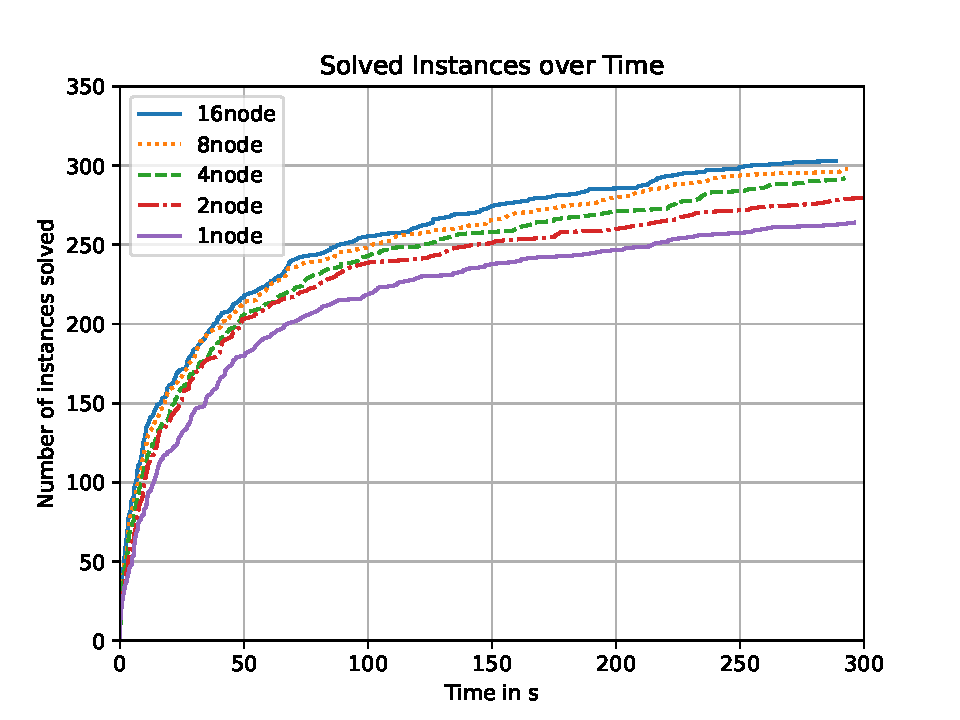
\includegraphics[scale=.8]{plots/cumulative_runtime/scalability_gim.pdf}\\
        Scalability of our approach with only Gimsatul as solver enigines
    \end{minipage}
    \hfill
    \begin{minipage}{0.45\textwidth}
        \center
        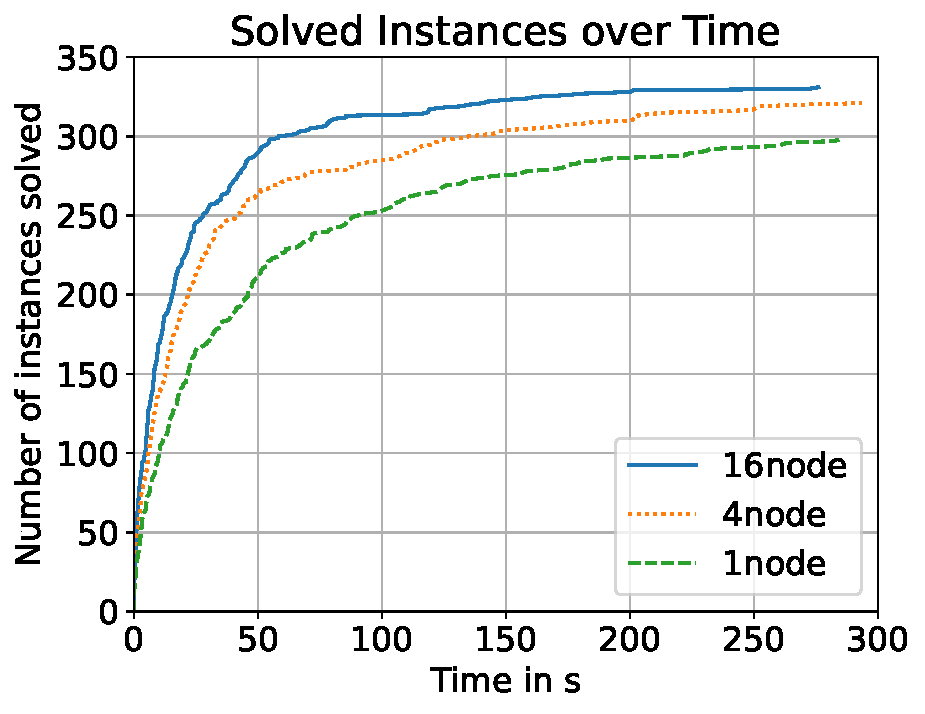
\includegraphics[scale=.8]{plots/cumulative_runtime/scalability_kis.pdf}\\
        Scalability of MallobSat with only Kissat as solver engines%' default configuration
    \end{minipage}
\end{frame}

\begin{frame}{Comparison to MallobSat -- Runtime}
    \begin{minipage}{.45\textwidth}
        \center
        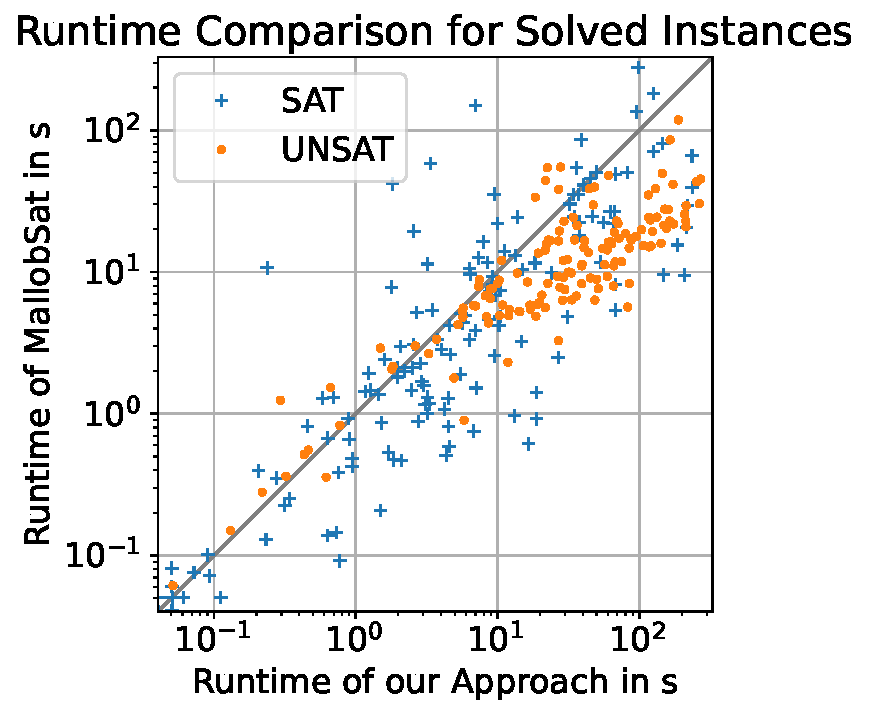
\includegraphics[scale=.8]{plots/square_runtime_compare/square_runtime_16node.pdf}\\
    \end{minipage}
    \hfill
    \begin{minipage}{.45\textwidth}
        \begin{itemize}
            \item \textcolor{gray}{x-axis: Our approach with only Gimsatul as solver enigines}
            \item \textcolor{gray}{y-axis: MallobSat with only Kissat as solver engines}
            \item \textcolor{gray}{log scale}
        \end{itemize}
        %Runtime Comparison between MallobSat and our approach, using 16 nodes.
    \end{minipage}
\end{frame}

\begin{frame}{Comparison to MallobSat -- Memory Consumption}
    \begin{minipage}{.45\textwidth}
        \center
        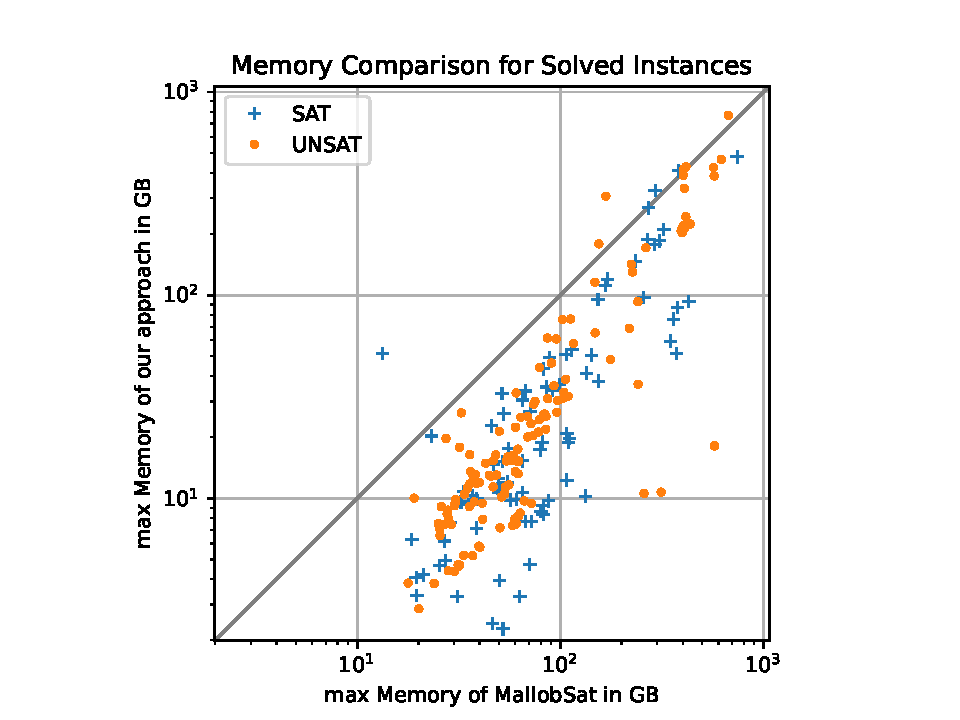
\includegraphics[scale=.8]{plots/square_mem_compare/square_mem_16node.pdf}\\
    \end{minipage}
    \hfill
    \begin{minipage}{.45\textwidth}
        \begin{itemize}
            \item \textcolor{gray}{x-axis: Our approach with only Gimsatul as solver enigines}
            \item \textcolor{gray}{y-axis: MallobSat with only Kissat as solver engines}
            \item \textcolor{gray}{log scale}
        \end{itemize}
        %Memory Comparison between MallobSat and our approach, using 16 nodes.
    \end{minipage}
\end{frame}

\begin{frame}{Comparison to MallobSat -- Memory Ratios}
    \begin{minipage}{.45\textwidth}
        \center
        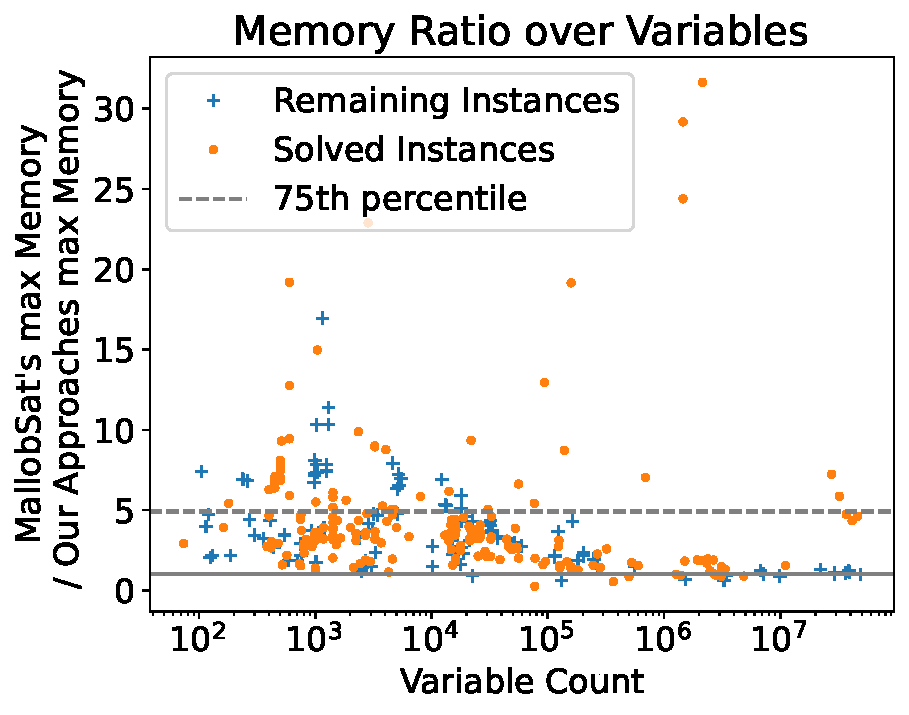
\includegraphics[scale=.8]{plots/16node_compare/mem_ratio_over_vars.pdf}\\
    \end{minipage}
    \hfill
    \begin{minipage}{.45\textwidth}
        \begin{itemize}
            \item \textcolor{gray}{Our Approach with only Gimsatul as solver engines}
            \item \textcolor{gray}{MallobSat with only Kissat as solver engines}
            \item \textcolor{gray}{Experiments on 16 nodes (768 cores)}
            \item \textcolor{gray}{Each data point corresponds to a benchmark instance}
        \end{itemize}
        %Memory ratios between MallobSat and our approach, using 16 nodes. Each data point corresponds to a benchmark instance.
    \end{minipage}
\end{frame}

\begin{frame}{Comparison to MallobSat -- Memory Geometric Mean}
    \begin{minipage}{.45\textwidth}
        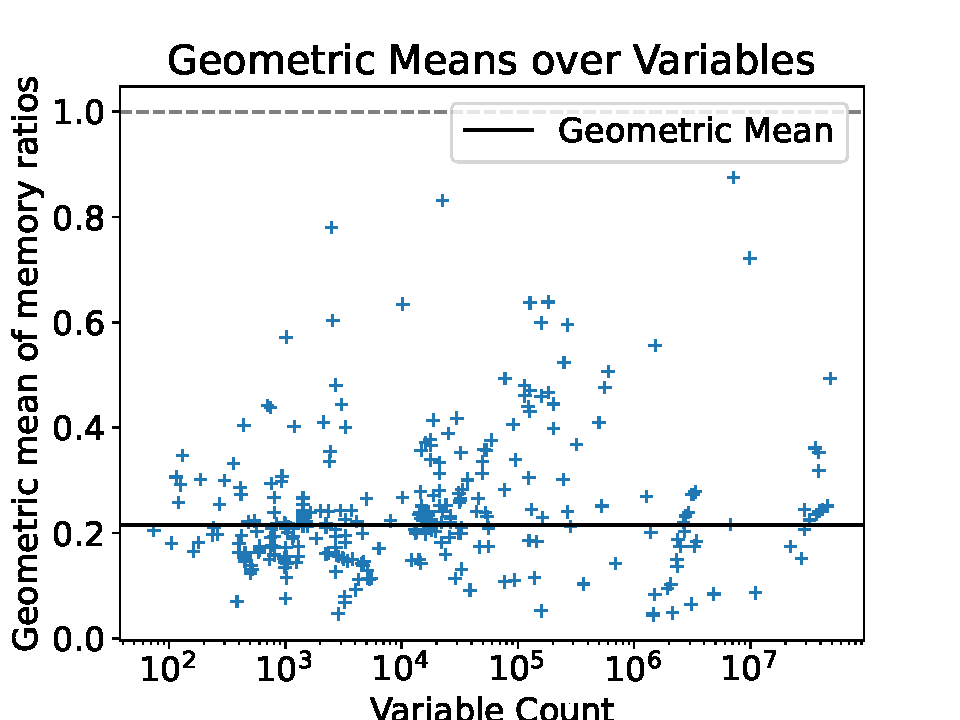
\includegraphics[scale=.8]{plots/16node_compare/mem_gm_over_vars.pdf}    
    \end{minipage}
    \hfill
    \begin{minipage}{.45\textwidth}
        \begin{itemize}
            \item \textcolor{gray}{Our Approach with only Gimsatul as solver engines}
            \item \textcolor{gray}{MallobSat with only Kissat as solver engines}
            \item \textcolor{gray}{Geometric mean ratiso between MallobSats default configuration and our Approach per second}
        \end{itemize}
        %Geometric means for memory ratios between MallobSat and our approach per second, using 16 nodes. Each data point corresponds to a benchmark instance.
    \end{minipage}
\end{frame}

\begin{frame}{Comparison to MallobSat -- Ratios per Second}
    \begin{minipage}{.45\textwidth}
        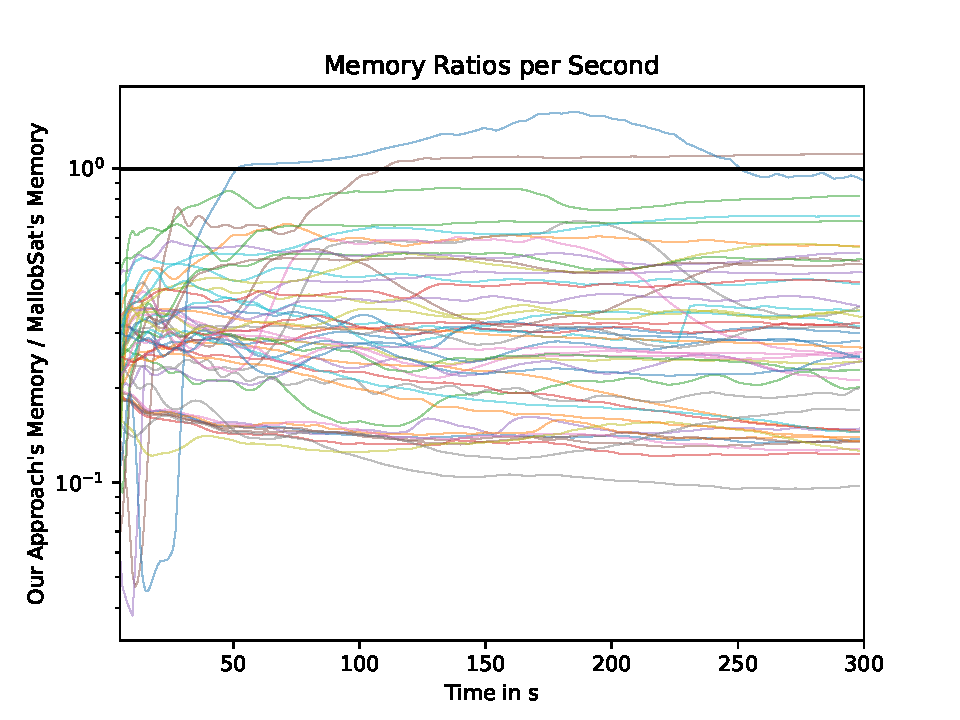
\includegraphics[scale=.8]{plots/16node_compare/mem_ratio_per_second.pdf}
    \end{minipage}
    \hfill
    \begin{minipage}{.45\textwidth}
        \begin{itemize}
            \item \textcolor{gray}{Our Approach with only Gimsatul as solver engines}
            \item \textcolor{gray}{MallobSat with only Kissat as solver engines}
            \item \textcolor{gray}{Memory ratios per second for all instances that reached the timeout of $300\,$s}
        \end{itemize}
        % (both with MallobSat and our approach), using 16 nodes. % The lines were smoothed, using a sliding window of size five seconds and calculating its geometric mean.
    \end{minipage}    
\end{frame}

\begin{frame}{Comparison to MallobSat -- Solved per Memory}
    \center
    \begin{table}%[scale=1.5]
        \center
        \begin{tabular}{ ccccc }
          \toprule
          \multicolumn{1}{c}{} & \multicolumn{2}{c}{Overall Used Memory} & \multicolumn{2}{c}{Normalized}\\
          \#cores & Our Approach & MallobSat & Our Approach & MallobSat \\
          \midrule
          48  & 0.149 & 0.089 & 7.140 & 4.256\\
          96  & 0.076 & -     & 7.306 & -\\
          192 & 0.039 & 0.026 & 7.583 & 5.036\\
          384 & 0.020 & -     & 7.780 & -\\
          768 & 0.010 & 0.006 & 7.766 & 4.924\\
          \bottomrule
        \end{tabular}
    \end{table}
    \vfill
    \textcolor{gray}{Solved instances per GB of used Memory}
    %Solved instances per GB of overall used memory in the middle and the same values normalized by the number of cores on the right.
\end{frame}

\begin{frame}{Interesting Tidbits}
    \centering
    \begin{table}[!h]
        \center
        \begin{tabular}{ lcccccc }
            \toprule
            family	&	\#	&	1node	&	2node	&	4node	&	8node	&	16node\\
            \midrule
            heule-folkman	&	11	&	0.425	&	-	&	0.416	&	0.449	&	0.444\\
            cryptography-simon	&	10	&	0.221	&	0.234	&	0.227	&	0.2	&	0.18\\
            miter	&	47	&	1.705	&	1.835	&	1.997	&	2.25	&	2.013\\
            \vdots &&&&&&\\
            % random-circuits	&	15	&	2.598	&	3.095	&	3.527	&	3.849	&	3.839\\
            % planning	&	6	&	2.567	&	3.977	&	4.168	&	4.623	&	4.835\\
            % software-verification	&	15	&	2.564	&	5.073	&	4.248	&	4.57	&	4.71\\
            % tseitin-formulas	&	8	&	4.442	&	4.567	&	5.177	&	5.275	&	5.49\\
            % hardware-verification	&	5	&	4.621	&	5.369	&	5.556	&	6.036	&	6.161\\
            % scheduling	&	50	&	5.333	&	6.434	&	7.944	&	8.384	&	8.799\\
            % heule-nol	&	11	&	5.988	&	11.793	&	7.786	&	10.231	&	12.876\\
            % cryptography-ascon	&	6	&	7.396	&	8.273	&	10.115	&	8.709	&	14.008\\
            % maxsat-optimum	&	13	&	7.419	&	7.32	&	12.362	&	13.762	&	14.899\\
            % quantum-kochen-specker	&	10	&	9.356	&	11.237	&	11.186	&	11.137	&	11.005\\
            % cryptography	&	7	&	6.32	&	16.922	&	9.289	&	21.402	&	23.632\\
            % hamiltonian	&	40	&	8.968	&	14.409	&	19.398	&	23.315	&	26.351\\
            % argumentation	&	21	&	13.01	&	16.268	&	18.577	&	21.941	&	20.716\\
            independent-set	&	15	&	16.442	&	18.038	&	20.981	&	27.173	&	25.9\\
            minimum-disagreement-parity	&	17	&	40.311	&	22.119	&	24.766	&	46.884	&	58.316\\
            rbsat	&	5	&	47.606	&	64.654	&	76.039	&	186.204	&	221.286\\
            \bottomrule
        \end{tabular}
    \end{table}
    \vfill
    %Geometric mean speedups per family and setup, for families comprising at least 5 instances and a calculatable speedup.
\end{frame}

%%%%%%%%%%%%%%%%%%%%%%%%%%%%%%%%%%%%

\section{Conclusion}
\begin{frame}{Conclusion}
    \begin{block}{Summary}
        \begin{itemize}
            \item Integrated Gimsatul into MallobSat as solver engine
            \item Evaluated approach
        \end{itemize}
    \end{block}

    \begin{block}{Conclusion}
        \begin{itemize}
            \item Succeeded in stated goal to increase memory-efficiency
            \item Elevator Pitch: \textbf{4x less memory} than default configuration
            \begin{itemize}
                \item gm of gm of Memory Ratios between MallobSat's default configuration and our approach is 0.25
            \end{itemize}
            \item Runtime tradeoff
        \end{itemize}
    \end{block}
\end{frame}

\end{document}
